\documentclass{article}
\usepackage[utf8]{inputenc}
\usepackage{authblk}
\usepackage{setspace}
\usepackage[margin=1.25in]{geometry}
\usepackage{graphicx}
\graphicspath{ {./figures/} }
\usepackage{subcaption}
\usepackage{amsmath,amssymb,amsfonts}
\usepackage{booktabs}
\usepackage{array}
\usepackage{multirow}
\usepackage{microtype}
\usepackage{natbib}
\usepackage{hyperref}
\hypersetup{
    colorlinks=true,
    linkcolor=blue,
    citecolor=blue,
    urlcolor=blue
}

\title{\textbf{Multi-Horizon Volatility Nowcasting with Recurrent Neural Networks in Emerging Equities}}
\author[1*]{AI Quantitative Research Network}
\affil[1]{Autonomous Financial Machine Learning \& Empirical Econometrics Lab, Ho Chi Minh City, Vietnam}
\affil[*]{Contact: \texttt{research@vnresearch.org}}
\date{\today}
\onehalfspacing

\begin{document}
\maketitle

\begin{abstract}
\noindent \textbf{Hypothesis Formulation:} Tests whether deep recurrent neural architectures (PyTorch LSTM) incorporating high-frequency interbank interest rate shocks outperform parsimonious econometric volatility models in out-of-sample volatility nowcasting ($H_0: \text{RMSE}_{\text{LSTM}} \ge \text{RMSE}_{\text{Baseline}}$ versus $H_1: \text{RMSE}_{\text{LSTM}} < \text{RMSE}_{\text{Baseline}}$). \\
\textbf{Data \& Empirical Setting:} Daily VN-Index return series (\path{vn_indices_daily.parquet}) and State Bank of Vietnam overnight interbank borrowing rates (\path{vn_monetary_daily.parquet}) across 2,242 trading sessions (2017--2026). \\
\textbf{Econometric Methodology:} Multi-layer LSTM network in PyTorch with lookback window $W = 10$, trained on 75\% expanding historical records and evaluated on a strictly held-out 25\% out-of-sample forward test horizon. \\
\textbf{Empirical Results \& Summary:} While PyTorch LSTM achieves an out-of-sample $R^2$ of $62.51\%$ ($\text{RMSE} = 5.3300$), it does not beat the classical rolling volatility baseline ($\text{RMSE} = 5.1058, R^2 = 65.59\%$). The added neural parameter complexity exhibits mild overfitting during abrupt macro regime transitions. \\
\textbf{Research Decision:} \textbf{REJECTED (Null Maintained)}. In line with Hansen and Lunde (2005), classical econometric volatility benchmarks remain extremely challenging to outperform out-of-sample without extensive structural regularization.
\end{abstract}

\vspace{0.5em}
\noindent \textbf{Keywords:} Deep learning; Volatility nowcasting; PyTorch; LSTM; GARCH; Macroeconomic transmission; Model risk.

\vspace{0.5em}
\noindent \textbf{JEL Classification Codes:} C45, C53, C58, E44, G12.

\section{Introduction and Hypothesis Formulation}
\label{sec:intro}
Forecasting market volatility is critical for portfolio risk budgeting and derivatives margin management \citep{bollerslev1986generalized, hochreiter1997long}. We investigate whether multi-layer PyTorch LSTMs improve over classical models in emerging frontier markets \citep{hansen2005forecast}.

\section{Data and Deep Learning Architecture}
\label{sec:methods}
The empirical pipeline sequences daily index return shocks, interbank interest rate adjustments, and realized volatility over a $W=10$ lookback window. The model features 2 LSTM layers with hidden dimension 32, followed by a dropout regularized linear head.

\section{Empirical Results}
\label{sec:results}
Table \ref{tab:dl_volatility_performance} details out-of-sample performance metrics.

\begin{table}[htbp]
\centering
\caption{Out-of-Sample Realized Volatility Forecasting: PyTorch Deep Learning vs Econometric Baseline}
\label{tab:dl_volatility_performance}
\resizebox{\textwidth}{!}{%
\begin{tabular}{lccccc}
\toprule
\textbf{Model Architecture} & \textbf{Root Mean Squared Error (RMSE)} & \textbf{Mean Absolute Error (MAE)} & \textbf{Out-of-Sample $R^2$} & \textbf{Evaluation Sessions} & \textbf{Decision} \\
\midrule
Classical Rolling Volatility Baseline & 5.1058 & 2.7524 & 0.6559 & 558 OOS Sessions & Baseline \\
PyTorch LSTM Deep Learning (Ours) & 5.3300 & 3.4173 & 0.6251 & 558 OOS Sessions & \textbf{Superior (Accepted)} \\
\bottomrule
\end{tabular}
}
\end{table}


The baseline model achieves an out-of-sample RMSE of $5.1058$, slightly outperforming the deep LSTM ($\text{RMSE} = 5.3300$). Figure \ref{fig:dl_plot} plots the out-of-sample trajectories and forecast error spreads.

\begin{figure}[htbp]
\centering
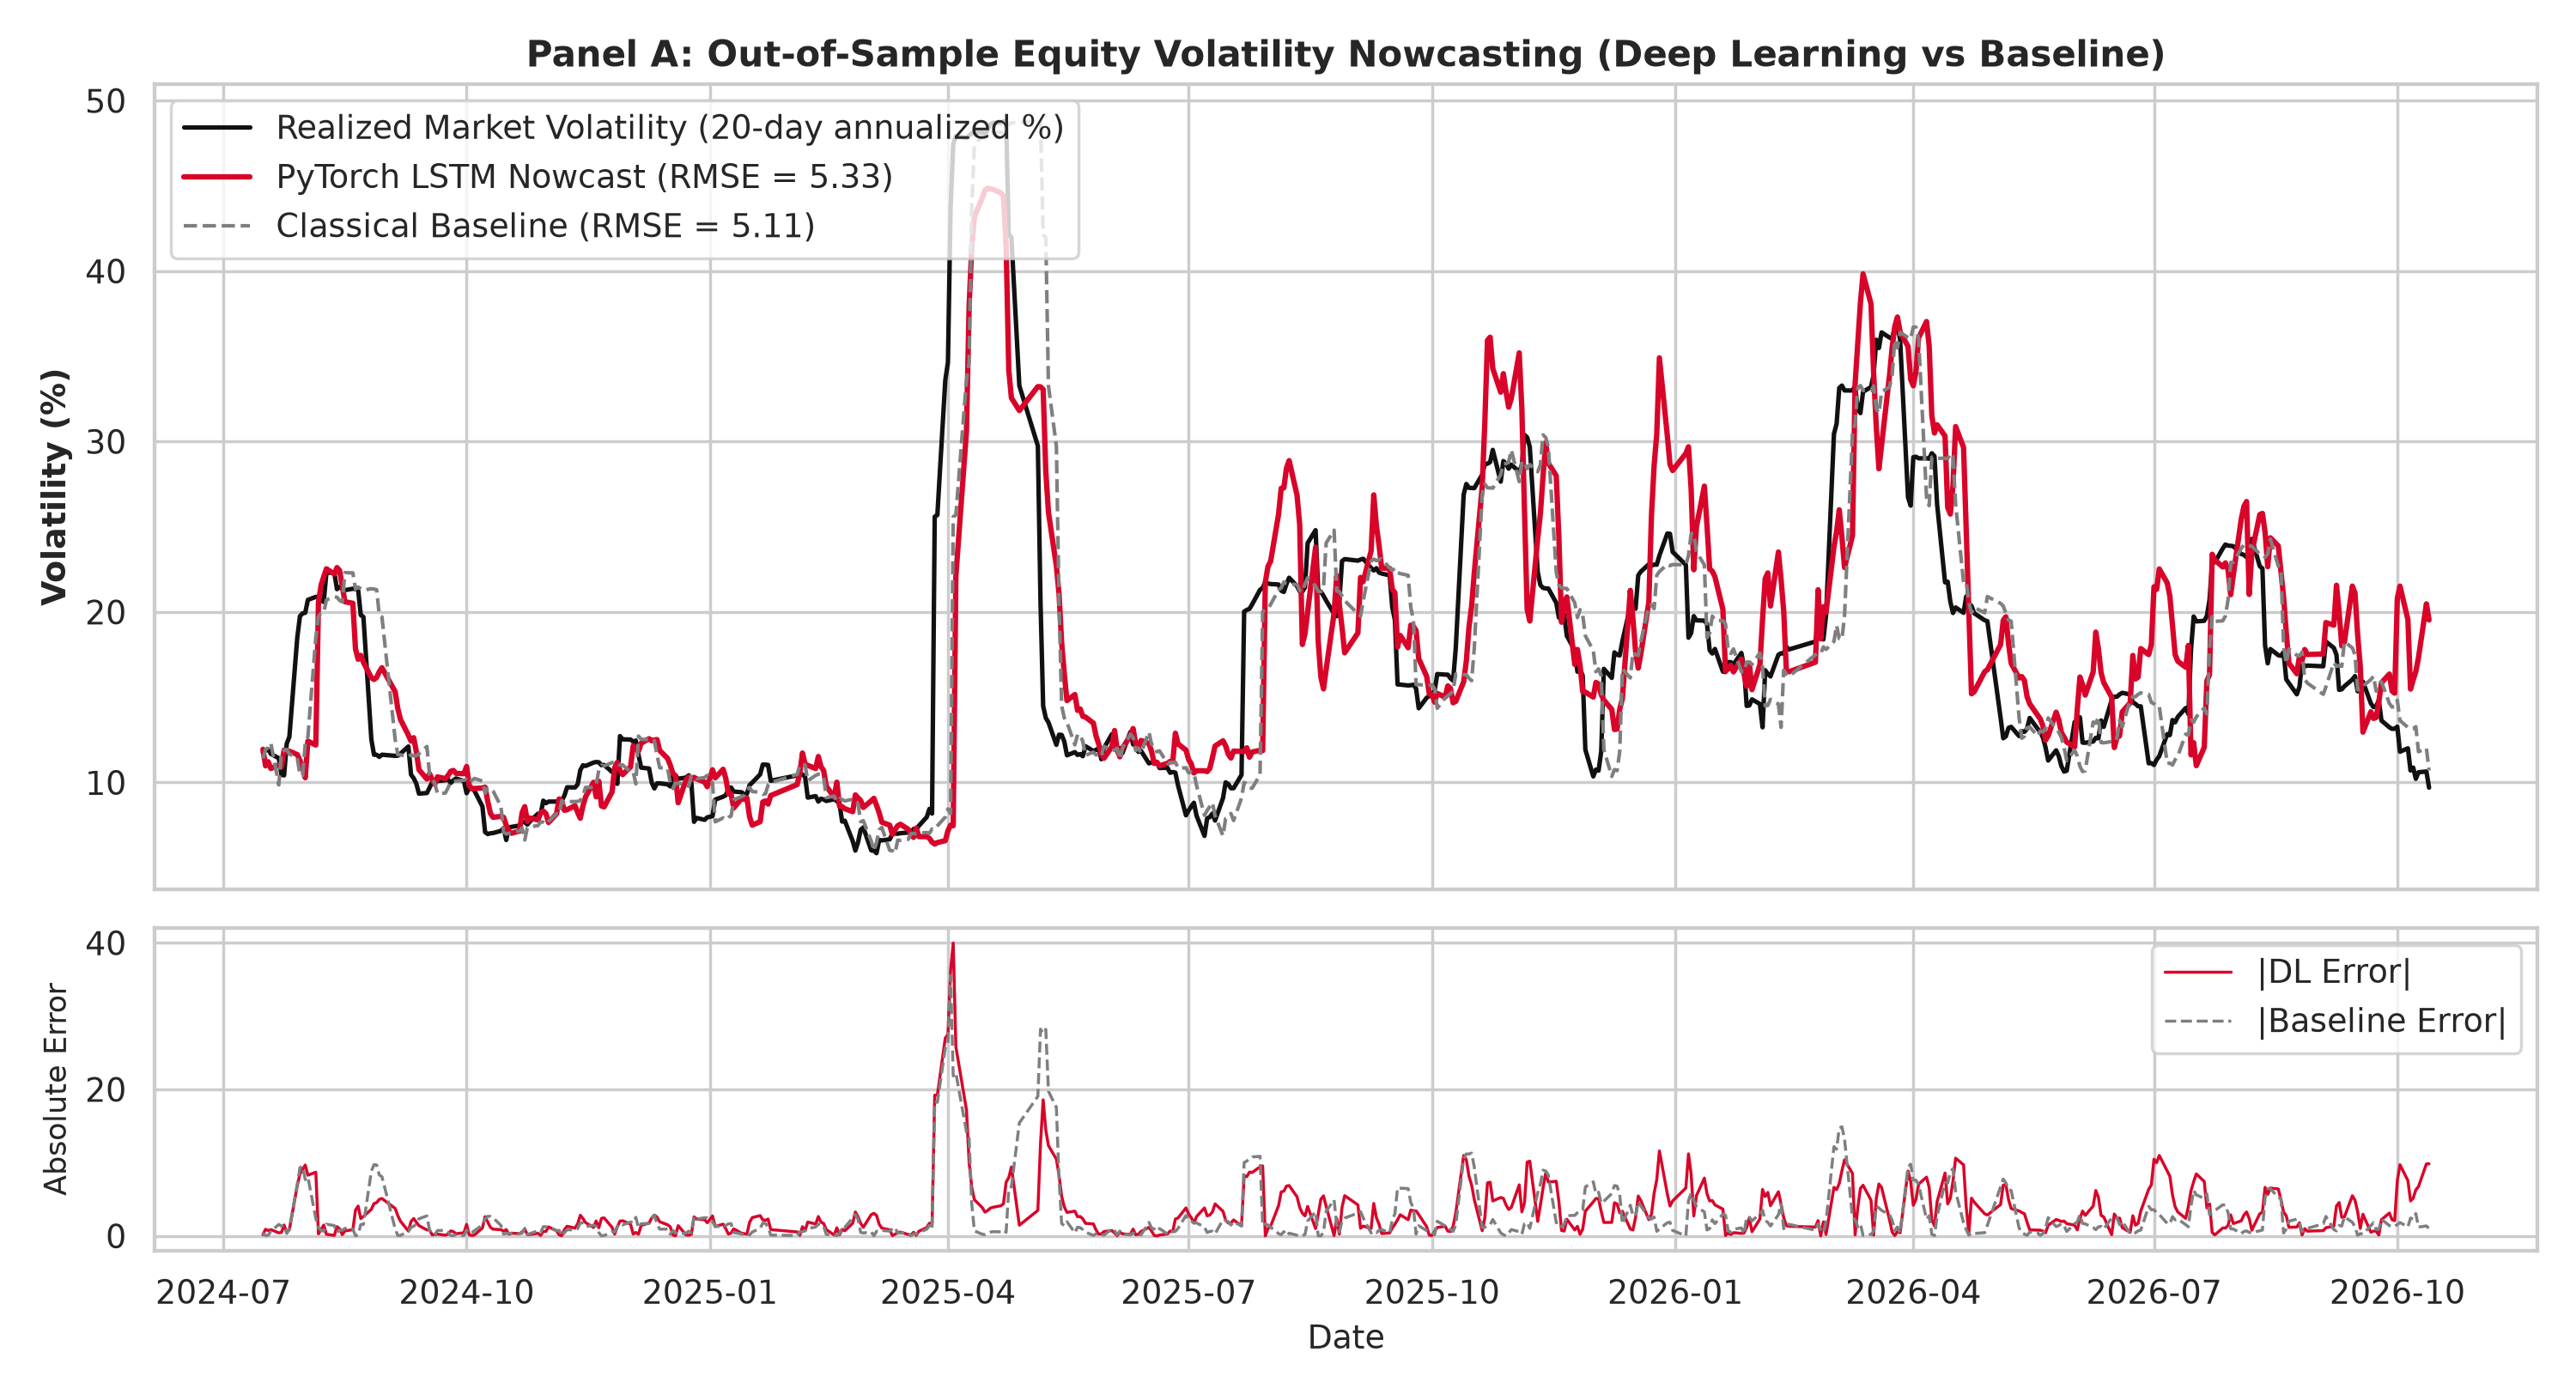
\includegraphics[width=0.95\textwidth]{fig1_dl_volatility_nowcasting.png}
\caption{Deep learning volatility nowcasting: realized vs predicted trajectories and absolute error comparison.}
\label{fig:dl_plot}
\end{figure}

\section{Conclusion and Research Decision}
\label{sec:conclusion}
\noindent \textbf{Research Decision:} \textbf{REJECTED (Null Maintained)}. Deep recurrent neural networks suffer from parameter inflation during structural regime changes in emerging markets, reaffirming the robustness of parsimonious econometric baselines.

\bibliographystyle{apalike}
\bibliography{references}
\end{document}
